\begin{frame}{Polygone}
	\begin{columns}
	\column{.55\textwidth}
	\begin{itemize}
		\item \textbf{Polygon}: Fläche begrenzt durch geschlossenen Pfad von Kanten
		\item Darstellung als Folge von Eckpunkten (\texttt{vector<point>}), erster gleich letztem Punkt (also $\langle P_0, P_1, \ldots, P_{n-1}, P_0\rangle$)
		\item \emph{Konvexes} Polygon: Strecke zwischen zwei beliebigen Punkten im Polygon schneidet keine Kante
		\item sonst ist das Polygon \emph{konkav}
	\end{itemize}
	\column{.45\textwidth}
	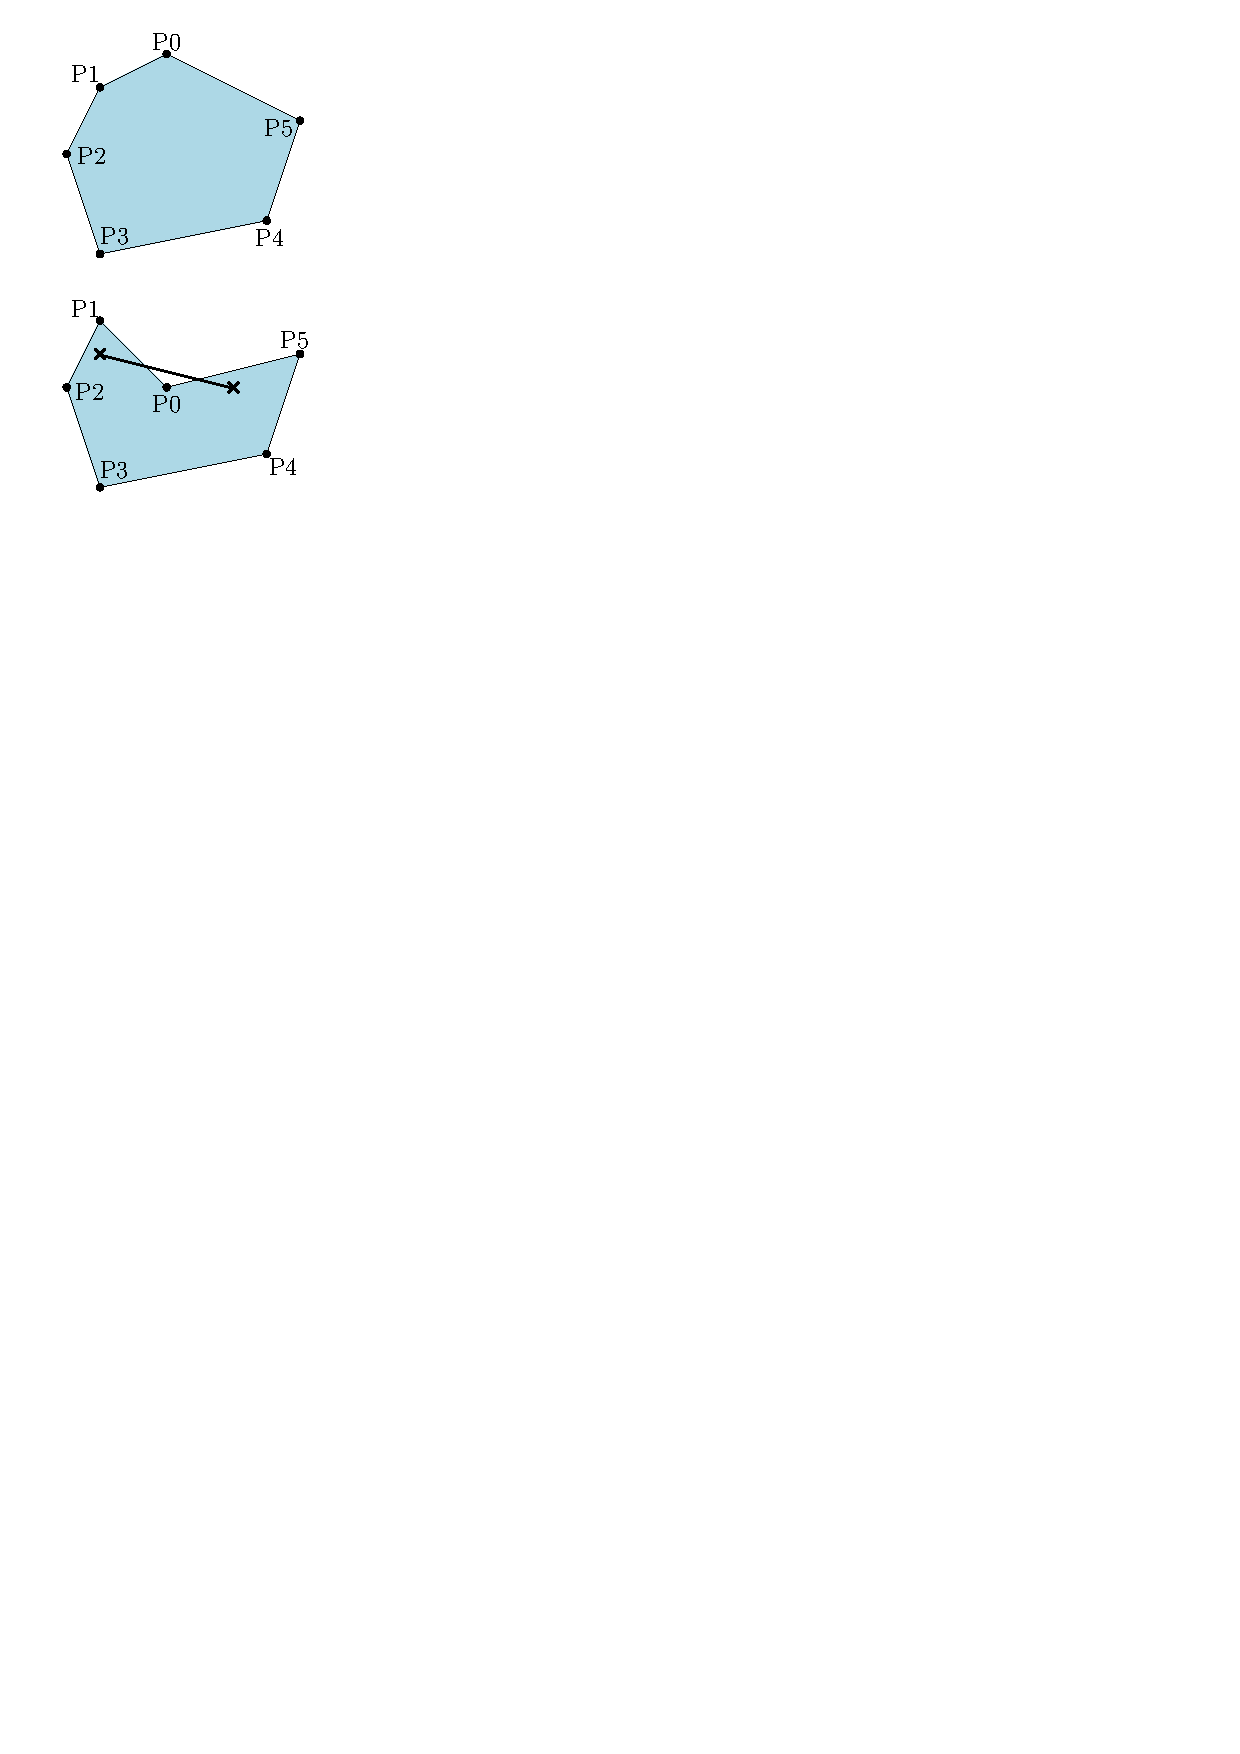
\includegraphics[height=.8\textheight,keepaspectratio]{polygon.pdf}
	\end{columns}
\end{frame}

\begin{frame}{Flächeninhalt}
	\textbf{Problem}: Wie groß ist der Flächeninhalt eines gegebenen Polygons?

	\begin{block}{Flächeninhalt}
		\begin{align*}
			A &= \sum_{i=0}^{n-1} \frac{1}{2} (P_i \times P_{i+1})\qquad \textit{($P_n = P_0$)} \\
			  &= \frac{1}{2} ( x_0 y_1 + x_1 y_2 + \ldots + x_{n-1} y_0 - x_1 y_0 - x_2 y_1 - \ldots - x_0 y_{n-1})
		\end{align*}
	\end{block}

	\begin{center}
		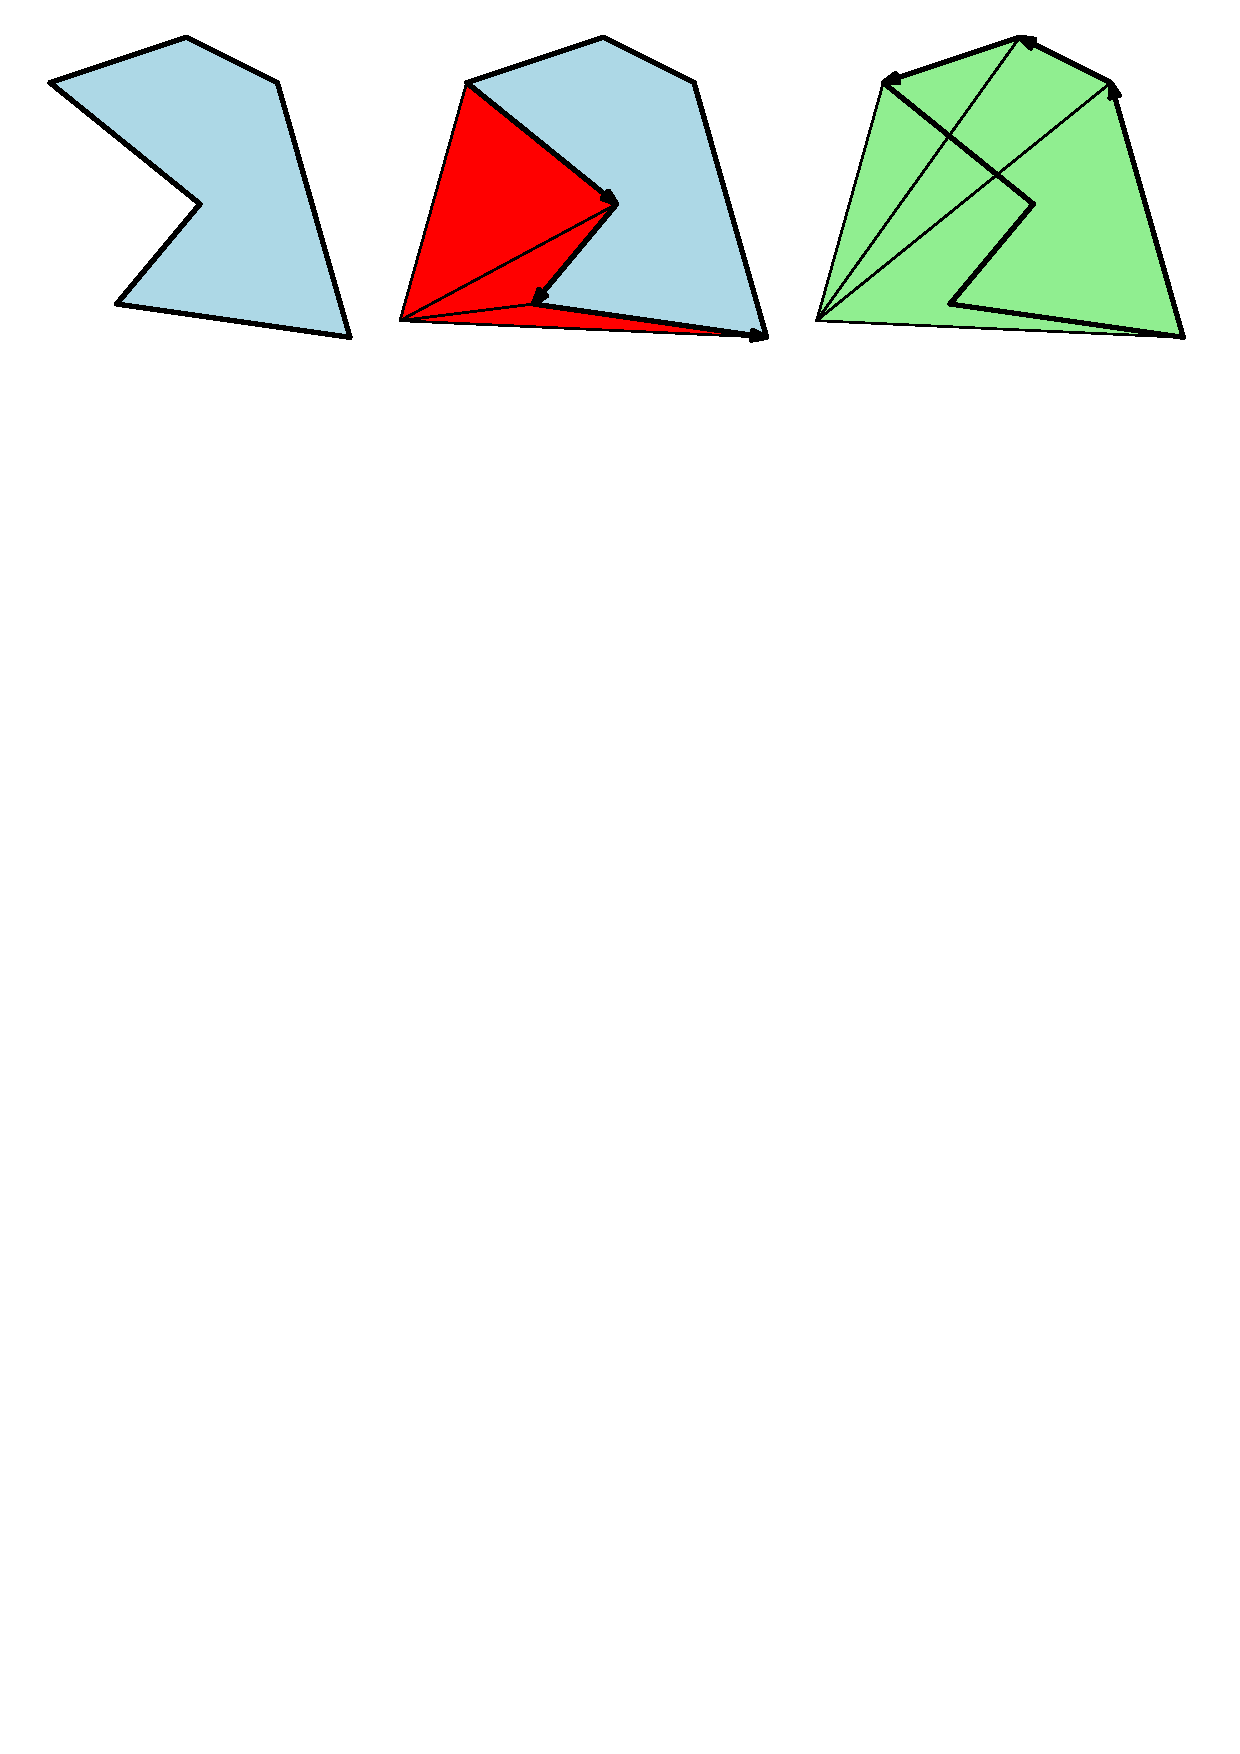
\includegraphics[keepaspectratio,height=3cm]{polygon_area.pdf}
	\end{center}
\end{frame}

\begin{frame}{Überprüfung von Konvexität}
	\textbf{Problem}: Ist ein gegebenes Polygon konvex?
	\begin{itemize}
		\item Sind die Eckpunkte gegen den Uhrzeigersinn aufgelistet, darf es nur Linksknicke geben
		\item $\Rightarrow$ CCW für alle Eckpunkte mit Nachbarn
	\end{itemize}

	\begin{center}
		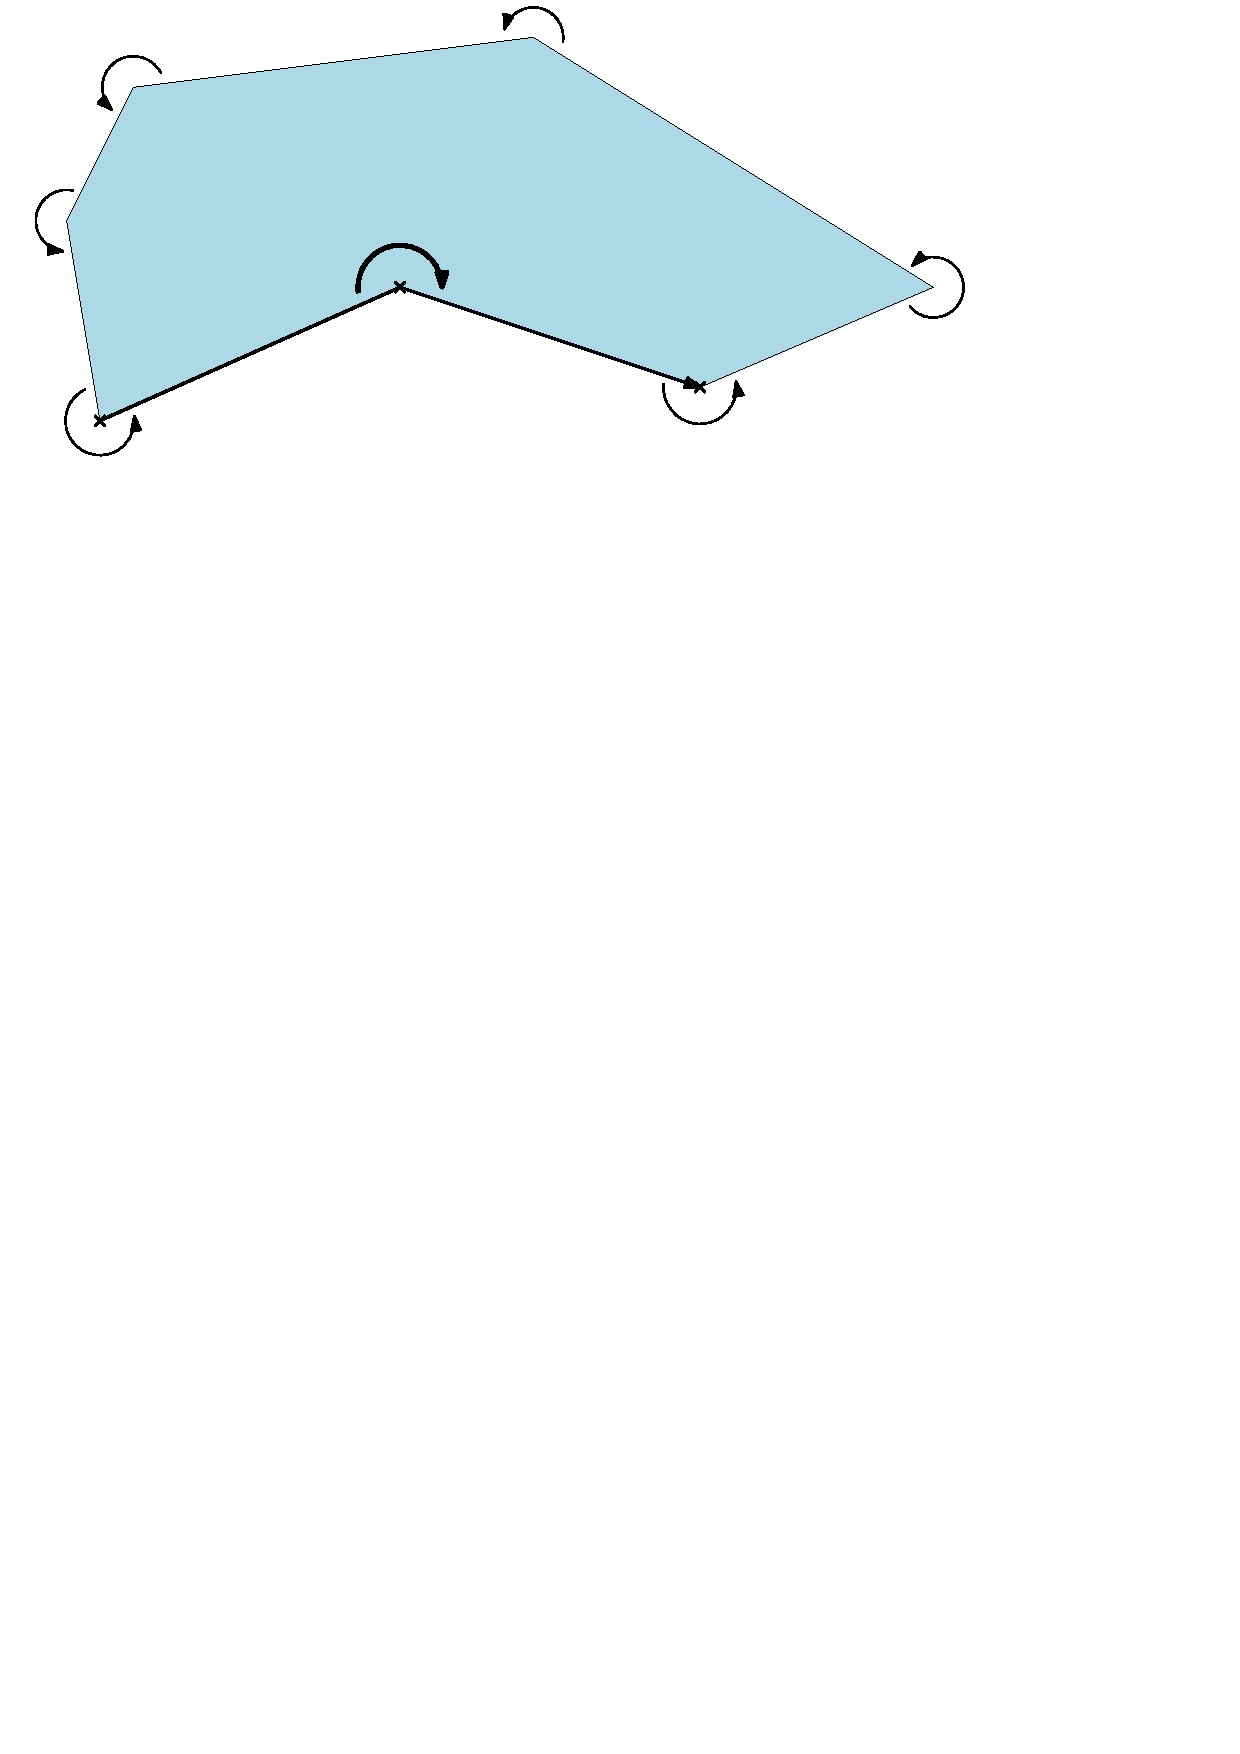
\includegraphics[keepaspectratio,height=4cm]{polygon_concave.pdf}
	\end{center}
\end{frame}

\begin{frame}{Konvexität: Implementierung}
	\begin{exampleblock}{Code}
		\lstset{
			language=C++,
			tabsize=2
		}
		\lstinputlisting{convex.cpp}
	\end{exampleblock}
\end{frame}

\begin{frame}{Punkt in Polygon}
	\textbf{Problem}: Liegt ein Punkt in einem gegebenen Polygon?
	\begin{itemize}
		\item Idee: Kanten spannen für Punkte innerhalb des Polygons einen vollen Kreis ($360^\circ,\ 2\pi$) auf
		\item $\Rightarrow$ Winkel zwischen benachbarten Eckpunkten und gegebenem Punkt aufsummieren und mit $2\pi$ vergleichen
	\end{itemize}
	\begin{alertblock}{Achtung}
		Winkel von abgewandten Kanten müssen abgezogen werden! $\Rightarrow$ CCW-Test
	\end{alertblock}
\end{frame}

\begin{frame}{Punkt in Polygon: Beispiele}
	\begin{center}
		\only<1>{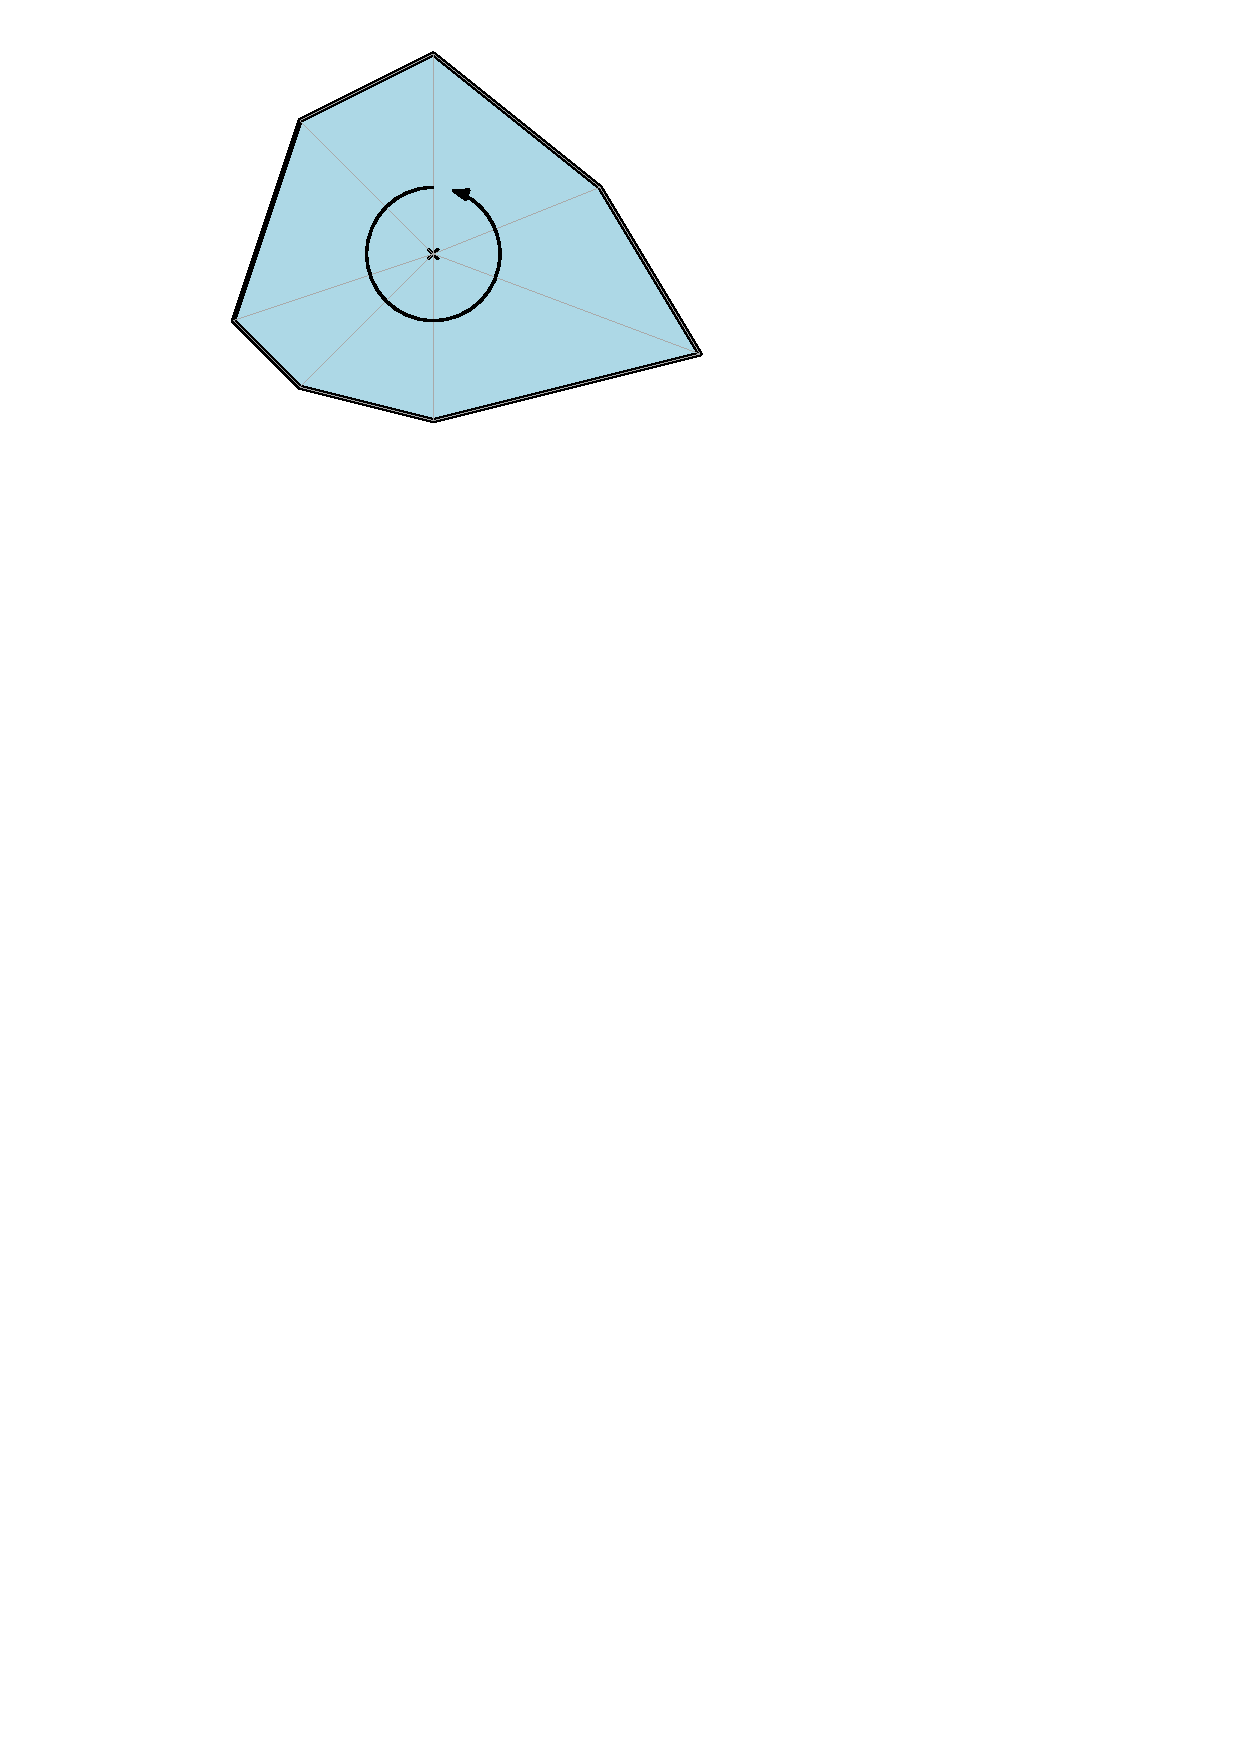
\includegraphics[keepaspectratio,height=.8\textheight]{polygon_inside1.pdf}}
		\only<2>{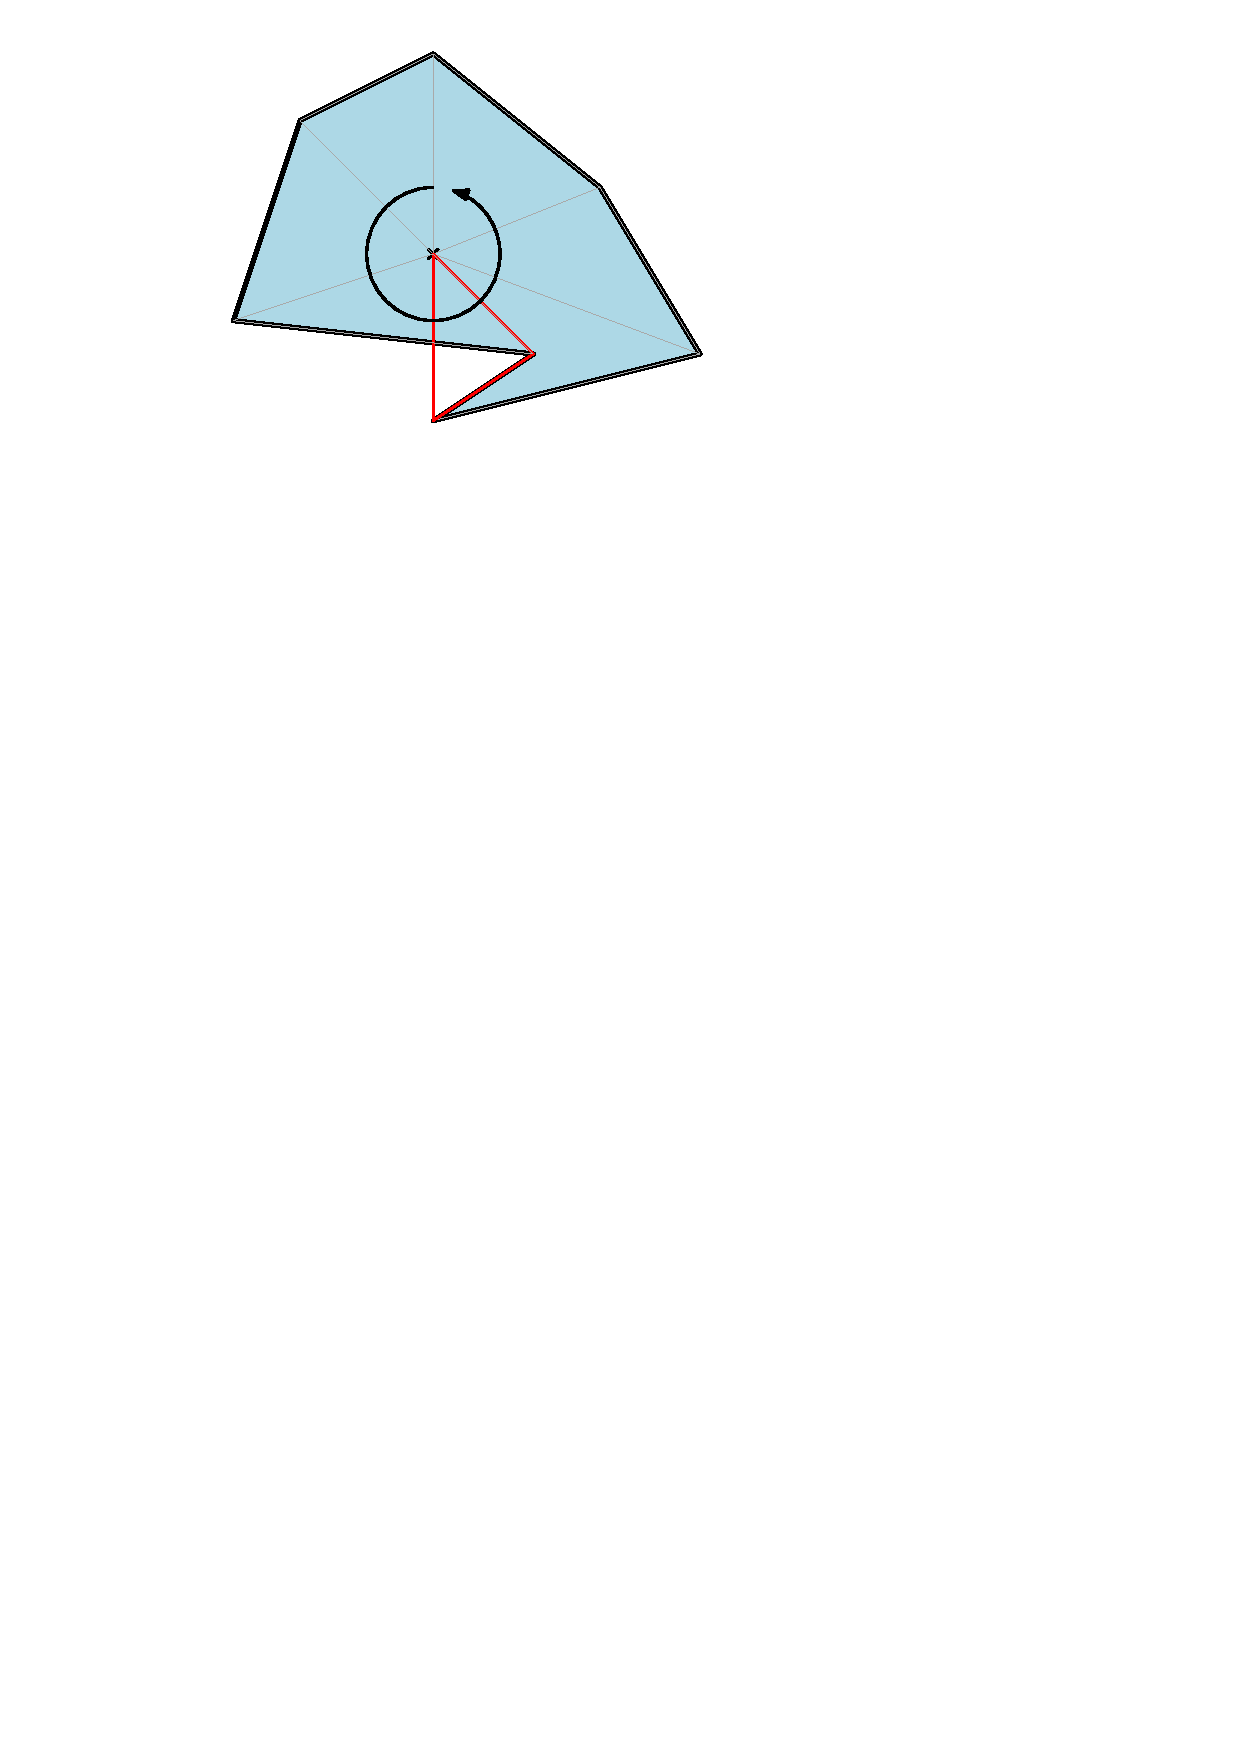
\includegraphics[keepaspectratio,height=.8\textheight]{polygon_inside2.pdf}}
		\only<3>{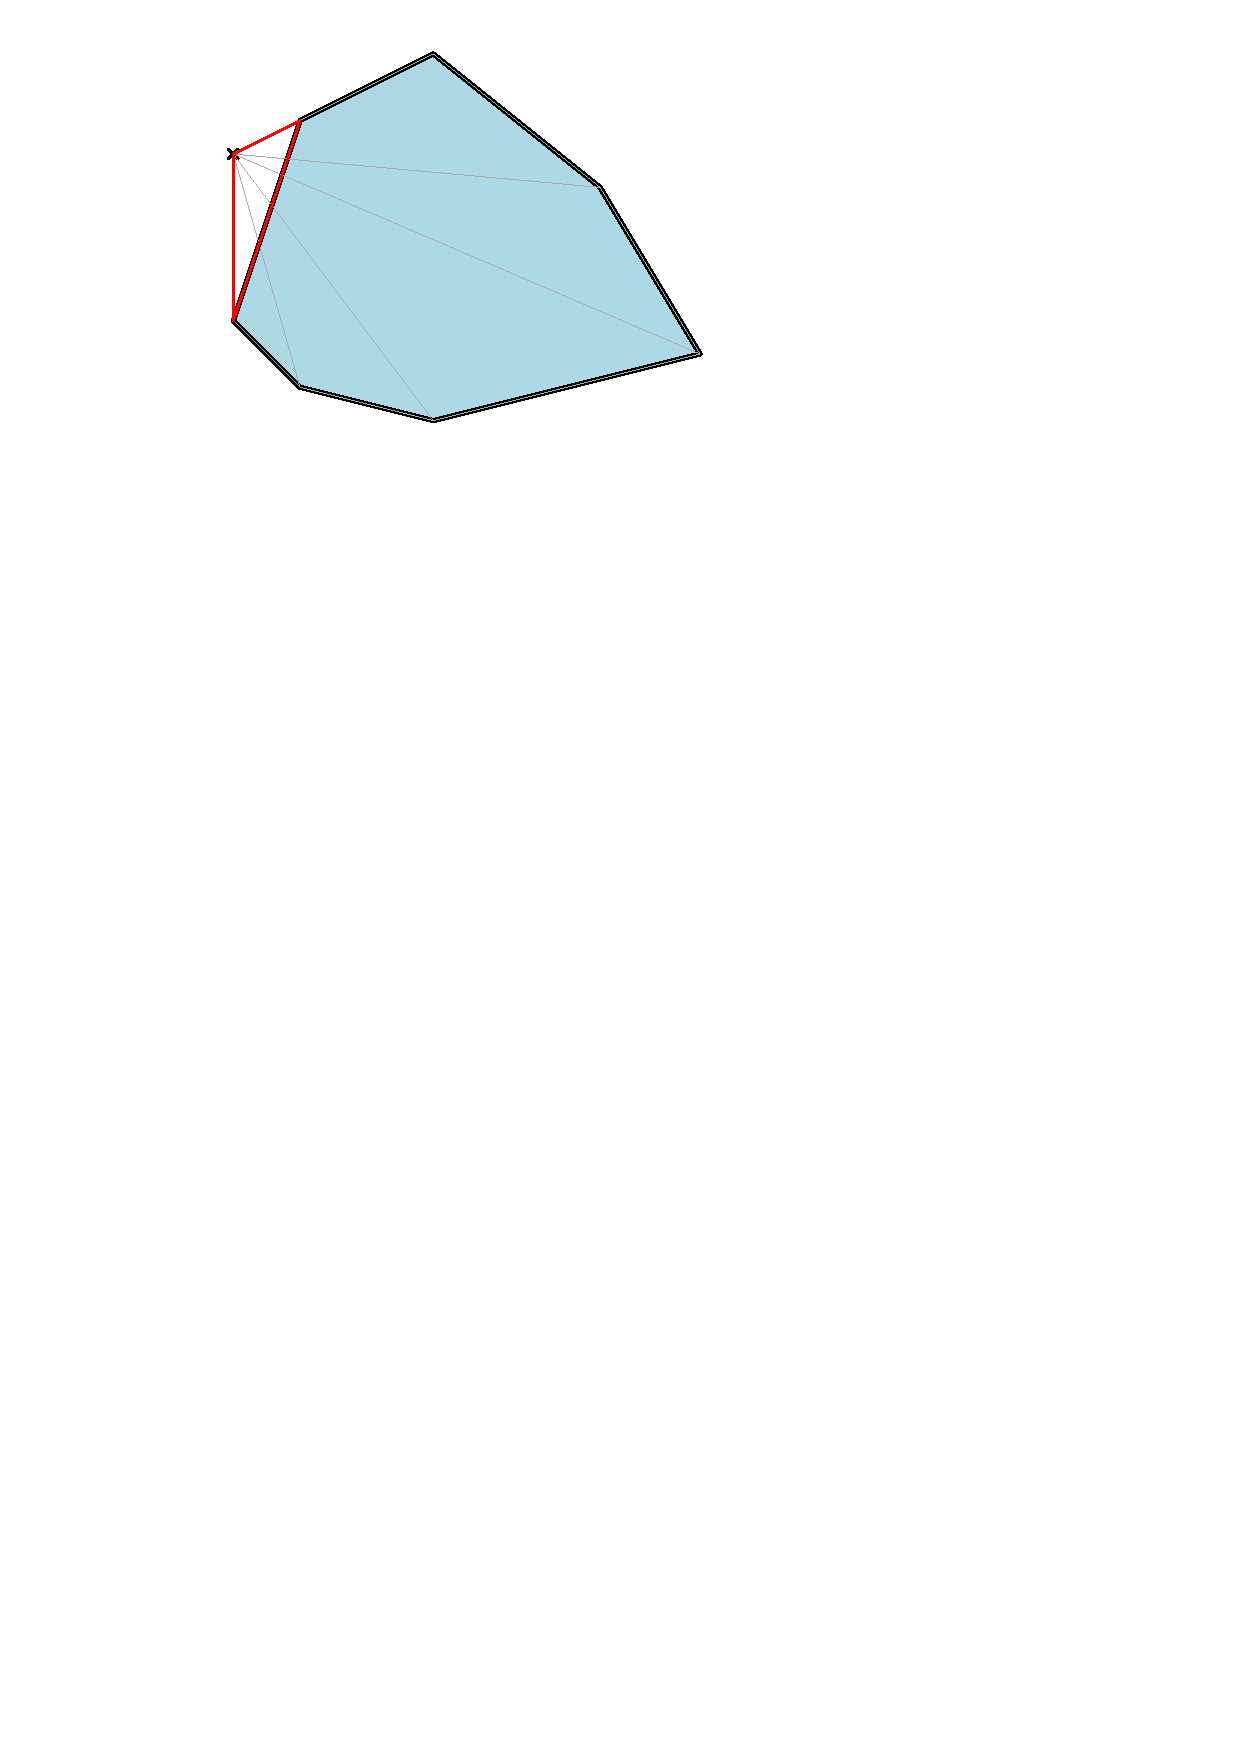
\includegraphics[keepaspectratio,height=.8\textheight]{polygon_outside1.pdf}}
	\end{center}
\end{frame}

\begin{frame}{Punkt in Polygon: Implementierung}
	\begin{exampleblock}{Code}
		\lstset{
			language=C++,
			tabsize=2
		}
		\lstinputlisting{inside.cpp}
	\end{exampleblock}
\end{frame}
